\section{Preliminaries}
\label{sec:prelim}
Let $\sigma = e_1, \ldots, e_m$ be the sequence of all edge insertions, and let $V$ be the set of vertices. 
We assume $m$ is of the form $2^k$ throughout this paper, which can be assumed without loss of generality by allowing dummy edge inserts.
Each edge $e_i$ has a weight $w(e_i) \in [1, W]$.
Let $G_t$ be the graph consisting of vertices $V$ and the first $t$ edges $e_1, \ldots, e_t$; we call this the \emph{graph at time $t$}. 
We define $G_0$ to be the empty graph on the vertex set $V$.

The \emph{length} of a path is the sum of the weights of its edges. 
Let $d^t(v)$ be the length of the shortest path from $s$ to $v$ in $G_t$. 
Throughout this paper, all logarithms are base 2 unless otherwise specified.

\paragraph{Problem Definition.}
In the offline problem, the algorithm is given a sequence of edge inserts $\sigma = e_1, e_2, \ldots, e_m$, the set of vertices $V$, and the source vertex $s$.  The goal of the algorithm is to output a data structure that answers queries $(v,t)$ of the form: what is the length of the shortest path from $s$ to $v$ at time $t$?  This answer should be a $(1 + \epsilon)$-approximation: specifically, for a query $(v, t)$, if the data structure returns $d$, then ${d}^t(v) \leq d \leq d^t(v)(1 + \epsilon)$.

In the online problem, the edges in $\sigma = e_1, \ldots, e_m$ arrive one at a time.  Before any edge arrives, the algorithm is given a prediction $\hat{\sigma}$ of $\sigma$, as well as the set of vertices $V=\{v_1,\ldots,v_n\}$ and the source vertex $s$.  
We assume the length of $\hat{\sigma}$ is the same as $\sigma$.
At all times, the algorithm must maintain an array $D$ containing the length of the shortest path to each vertex.  In particular, after edge $t$ is inserted, $D$ must satisfy $d^t(v_i)\leq D[i] \leq d^t(v_i)(1 + \epsilon)$ for all vertices $v_i$.

\paragraph{Adjusting $\epsilon$.}
Throughout this paper, we assume $\epsilon = O(1)$.
In our algorithms, distance estimates $\hat{d}^t(v)$ are used for each node $v$ and time $t$ that satisfy the following invariant (see Lemmas~\ref{lem:refined_approx} and~\ref{lem:pred_approx}):
$d^t(v) \leq \hat{d}^t(v) \leq d^t(v)(1 + \epsilon/ \log m)^{\log m}$.

We will need to slightly adjust $\epsilon$ in our algorithms to account for lower-order terms.
For $\epsilon<1.79$, it is known that
\[\left( 1 + \frac{\epsilon}{\log m}\right)^{\log m} \leq e^\epsilon \leq 1+\epsilon+\epsilon^2,\]
which ensures that $d^t(v) \leq \hat{d}^t(v) \leq d^t(v)(1 + \epsilon + \epsilon^2)$.
To ensure our algorithms return $(1+\epsilon)$ approximations for $d^t(v)$, the $\epsilon$ parameters used are set to be $(\min\{1.79,\epsilon\})/4$. 

\paragraph{Defining Recursive Subproblems.}
The offline algorithm is recursive.
It divides the interval $[0,m]$ in half and recurses on both sides. On each recursive call, the algorithm will process an interval $[\ell, r]$ and further subdivide the interval until it contains a single edge. 
We call each recursive call $[\ell,r]$ a \emph{subproblem}.
We refer to this subproblem both as \emph{subproblem $[\ell,r]$} and \emph{subproblem $x$}, where $x=(\ell+r)/2$ is the midpoint of $[\ell,r]$.
Each subproblem corresponds to a node in the recursion tree.
We might refer to the subproblem $[\ell,r]$ in the recursion tree as \emph{node $x$} in the recursion tree.
Each time $x \in \{1,\ldots,m-1\}$ is the midpoint of exactly one node in the tree.
Let the \defn{level} of a time $x$ be the depth of node $x$ in the recursion tree. 
So the level of $m/2$ is $1$, the level of $m/4$ and $3m/4$ is $2$, and so on.
In particular, the level of $x$ is one more than the maximum level of $\ell$ and $r$.
For ease of notation, we set the level of 0 and $m$ to be 0. 
See Figure~\ref{fig:tree} for an illustration of the recursion tree.
We refer to the ancestors and descendants of a node in the recursion tree as \emph{ancestors} and \emph{descendants} of the corresponding subproblem.
All these definitions extend to the online algorithm as well, as it is built up on the offline algorithm.


\begin{figure}
    \centering
    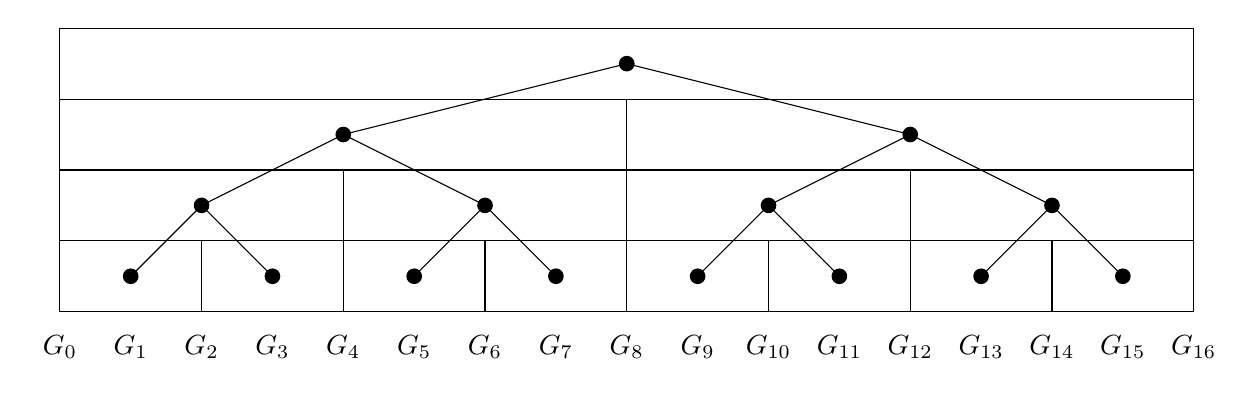
\begin{tikzpicture}[main/.style = {fill = black, circle, inner sep = 2pt}, 
    label/.style = {fill = none, circle, inner sep = 3pt}, 
    scale = 0.9]
        \draw[step = 1cm, gray, thin] (0,1) grid (16,5);
            \filldraw[fill = white, draw = black] (0,5) rectangle (16,4);
        \foreach \i in {0, 8}
            \filldraw[fill = white, draw = black] (\i,4) rectangle (\i+8,3); 
        \foreach \i in {0, 4, ..., 12}
            \filldraw[fill = white, draw = black] (\i,3) rectangle (\i+4,2);    
        \foreach \i in {0, 2, ..., 14}
            \filldraw[fill = white, draw = black] (\i,2) rectangle (\i+2,1);

        \foreach \i in {0, 1, 2, ..., 16}
            \node[label] at (\i, 0.5) {$G_{\i}$};
        
        \node[main] at (8, 4.5) {};
        \foreach \i in {4, 12}
            \node[main] at (\i, 3.5) {};
        \foreach \i in {2, 6, 10, 14}
            \node[main] at (\i, 2.5) {};
        \foreach \i in {1, 3, ..., 16}
            \node[main] at (\i, 1.5) {};
    
        \foreach \i in {4, 12}
           \draw (8, 4.5) -- (\i, 3.5);
        \foreach \i in {2, 6}
           \draw (4, 3.5) -- (\i, 2.5);
        \foreach \i in {10, 14}
           \draw (12, 3.5) -- (\i, 2.5);
        \foreach \i in {1, 3}
           \draw (2, 2.5) -- (\i, 1.5);
        \foreach \i in {5, 7}
           \draw (6, 2.5) -- (\i, 1.5);
        \foreach \i in {9, 11}
           \draw (10, 2.5) -- (\i, 1.5);
        \foreach \i in {13, 15}
           \draw (14, 2.5) -- (\i, 1.5);  
    \end{tikzpicture}    
    \vspace{-.15in}
    \caption{The recursion tree of the algorithm. Each node $x$ in the tree is associated with an interval $[\ell,r]$ such that $x=(\ell+r)/2$. The depth of a node is the number of nodes in the path from the root $m/2$ to that node. For example, the depth of node $x=6$ is 3, and its corresponding interval is $[4,8]$.}
    \label{fig:tree}
    \vspace{-.15in}
\end{figure}
